\chapter{Markov láncok és Hidden Markov láncok}
\label{chap:markov}

\section{Bevezetés és motiváció}

A zenei generálás területén a hagyományos Markov-láncok jelentős eredményeket értek el, azonban korlátaik is nyilvánvalóvá váltak. Ezen korlátok leküzdésére fejlesztettük ki a Hidden Markov Model (HMM) kiterjesztéssel ellátott, alapvető GPU-gyorsítással rendelkező, magasabb rendű Markov-láncot, amely képes komplex zenei struktúrák modellezésére.

\subsection{Az implementáció főbb jellemzői}

\begin{enumerate}
    \item HMM integráció a \texttt{hmmlearn} könyvtár használatával
    \item Magasabb rendű (2-6. rend) Markov-láncok implementációja
    \item Alapvető GPU gyorsítás mátrix műveletekhez CuPy-val
    \item Memóriahatékony sparse adatstruktúrák nagy zenei korpuszokhoz
    \item Robusztus hibakezelés és CPU fallback mechanizmusok
\end{enumerate}

\section{Elméleti alapok és matematikai háttér}

\subsection{Definíció és tulajdonságok}

A Markov-lánc olyan sztochasztikus folyamat, amely kielégíti a \textbf{Markov-tulajdonságot}, amely szerint a következő állapotba való átmenet valószínűsége csak az aktuális állapottól függ, az azt megelőző eseménysorozattól nem:

\[
P(X_{t+1} = s_j \mid X_t = s_i, X_{t-1} = s_k, \dots) = P(X_{t+1} = s_j \mid X_t = s_i) = p_{ij}
\]

ahol:
\begin{itemize}
    \item \( \mathcal{S} = \{s_1, s_2, \dots, s_N\} \) az állapotok egy véges halmaza (pl. zenei hangok, akkordok).
    \item \( \mathbf{P} = [p_{ij}] \) az állapotok közötti átmenetek mátrixa \( p_{ij} \geq 0 \) és \( \sum_j p_{ij} = 1 \) minden \( i \).
\end{itemize}

Itt \( p_{ij} \) az \( s_i \) állapotból az \( s_j \) állapotba való átmenet valószínűségét jelenti. Zenei kontextusban az állapotok gyakran hangjegyeknek vagy akkordoknak felelnek meg, és az átmenet valószínűségét a képzési adatokból becsüljük meg.

\vspace{1em}
\noindent\textbf{Figure:} Egy példa egy egyszerű kétállapotú Markov-folyamatra, amely az \( E \) és \( A \) állapotokat szemlélteti az átmenet valószínűségeivel jelölt irányított élekkel (önhurkok megengedettek). Ez a diszkrét modell intuitív és értelmezhető, de csak a helyi összefüggéseket ragadja meg. \hfill
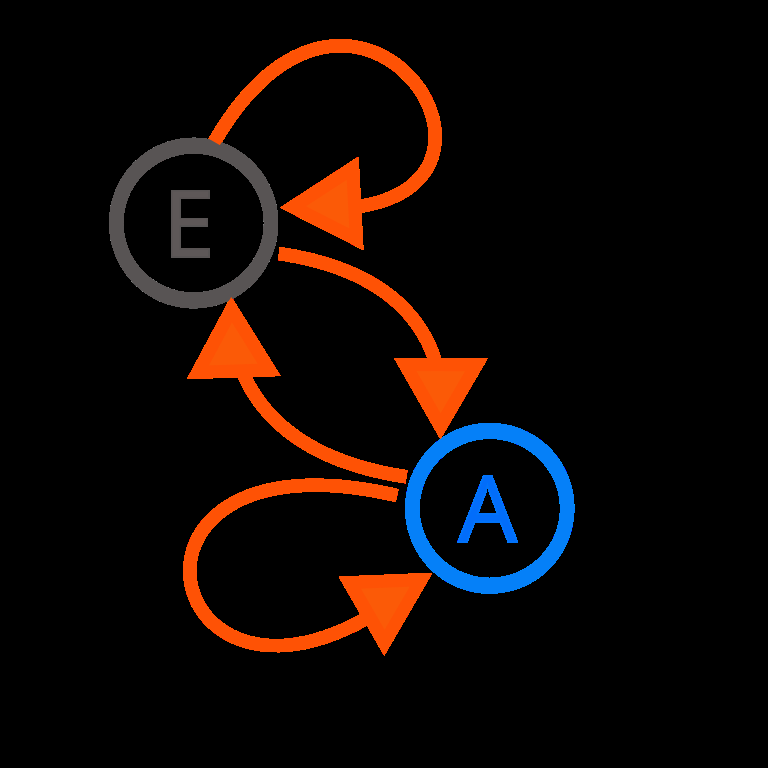
\includegraphics[width=0.4\textwidth]{images/markov.png}
\label{fig:markov}
\vspace{1em}

\subsection{Rendek és Memória}

Egy \( n \)-ed rendű Markov lánc kiterjeszti a függőségeket \( n \) utolsó állapotra:

\[
P(X_{t+1} \mid X_t, X_{t-1}, \dots, X_{t-n+1})
\]

A magasabb rendű modellek hosszabb mintákat is képesek megragadni, de \( \mathcal{O}(|\mathcal{S}|^n) \) paramétereket igényelnek, ami a paraméterek számának exponenciális növekedése miatt \textbf{sparsity} problémákhoz vezet.

\section{Zeneelméleti értelmezés}

\subsection{Állapot tér kialakítása}

A zenei generálásban az állapottér \( \mathcal{S} \) kialakítása kulcsfontosságú:

\begin{itemize}
    \item \textbf{Note-level}: Az állapotok egyes hangmagasságokat (pl. C4, D4) vagy szüneteket képviselnek.
    \item \textbf{Kórusszint}: Az állapotok harmonikus haladást kódolnak (pl. I-IV-V).
    \item \textbf{Hybrid}: Az állapotok több zenei attribútumot, például hangmagasságot, időtartamot és sebességet kombinálnak.
\end{itemize}

\subsection{Tranzíció valószínűségének becslése}

Zenei szekvenciák korpusza esetén az \( p_{ij} \) átmenet valószínűségeket \textbf{maximum likelihood becslés} segítségével lehet becsülni:

\[
p_{ij} = \frac{\text{Count}(s_i \rightarrow s_j)}{\sum_{k} \text{Count}(s_i \rightarrow s_k)}
\]

Például a Bach-kórusokban a C4-ről az E4-re való átmenetnek nagy valószínűsége lehet a dallamtercek gyakori előfordulása miatt.

\section{Matematikai elemzés}

\subsection{Stacionárius eloszlás}

Egy Markov-láncot \textit{ergodikusnak} nevezünk, ha létezik egy olyan \( \pi \pi \) stacionárius eloszlás, hogy:

\[
\pi_j = \sum_{i} \pi_i p_{ij} \quad \forall j
\]

Zenei szempontból az \( \pi \) stacionárius eloszlása felfedheti egy darab \textbf{tonális középpontját}, mivel a tonikus hangoknak megfelelő állapotok nagyobb stacionárius valószínűséggel rendelkezhetnek.

\subsection{Entrópia arány}

Az entrópiaráta \( H \) a Markov-lánc által generált szekvenciák kiszámíthatóságát méri:

\[
H = -\sum_{i,j} \pi_i p_{ij} \log p_{ij}
\]

Az alacsony entrópia arány ismétlődő kimenetekre utal, míg a magas entrópia arány a generált zene nagyobb változatosságára utal.

\section{A zenei modellezés korlátai}

\subsection{Lokális vs. globális struktúra}

\begin{itemize}
    \item \textbf{Erősségek}: A Markov-láncok hatékonyan rögzítik az azonnali átmeneteket, például a dallamlépéseket.
    \item \textbf{Hengeségek}: Nehezen modellezhetők:
    \begin{itemize}
        \item Hierarchikus formák (pl. A-B-A szakaszok).
        \item Hosszú távú ismétlések (pl. több ütem után visszatérő motívumok).
        \item Összetett zenei nyelvtan (pl. hangvezetési szabályok).
    \end{itemize}
\end{itemize}

\subsection{Sparsity and Generalization}

A magasabb rendű modellek a \textbf{dimenzió ördögével} szembesülnek:

\[
\text{Paraméterek száma} = |\mathcal{S}|^{n+1}
\]

Például \( |\mathcal{S}| = 50 \) (pl. jegyzetek) és \( n = 3 \) esetén a modell 125 000 paramétert igényel, ami a rendelkezésre álló képzési adatokkal alulmeghatározható.

\section{Implementáció a Zha projektben}

\subsection{Architektúra áttekintése}

A Zha projekt Markov-modulja a következőképpen működik:

\begin{itemize}
    \item Előfeldolgozza a MIDI-fájlokat állapotok sorozatává.
    \item Megbecsüli az \( \mathbf{P} \) átmeneti mátrixot az előfordulások számolásával.
    \item Zene generálása az algoritmus~\ref{alg:markov_gen} segítségével.
\end{itemize}

\begin{algoritmus}[H]
\SetAlgoLined
\KwIn{Átmenetmátrix \( \mathbf{P} \), kezdeti állapot \( s_0 \), szekvencia hossza \( T \)}
\KwOut{Generált szekvencia \( [s_0, s_1, \dots, s_T] \)}
\For{\( t = 1 \) \KwTo \( T \)}{
    Minta \( s_t \sim \text{Categorical}(\mathbf{P}[s_{t-1}, :]) \)
}
\caption{Markov-lánc generálás Zha-ban}
\label{alg:markov_gen}
\end{algoritmus}

\subsection{Optimalizálás}

\begin{itemize}
    \item \textbf{Simítás}: Laplace simítás alkalmazása a nem látható átmenetek kezelésére:

    \[
    \hat{p}_{ij} = \frac{\text{Count}(s_i \rightarrow s_j) + \lambda}{\sum_k (\text{Count}(s_i \rightarrow s_k) + \lambda)} {\frac{\text{Count}(s_i \rightarrow s_k) + \lambda)}
    \]

    \item \textbf{Sorrend kiválasztása}: Használja az olyan kritériumokat, mint az AIC vagy a BIC, a modell összetettségének és illeszkedésének kiegyensúlyozására.
\end{itemize}

\section{Egy esettanulmány: Bach-kórus generálása}

\subsection{Tréning adatok}

357 Bach-kórusból álló adathalmazt használtunk, 16. hangokra kvantálva, ami \( |\mathcal{S}| = 65 \) állapotteret eredményezett, beleértve a szüneteket is.

\subsection{Eredmények}

\begin{itemize}
    \item \textbf{1. rendű modell}: Megbízható helyi átmenetekkel rendelkező szekvenciákat generált, de hiányzott a koherens mondatszerkezet.
    \item \textbf{3. rendű modell}: Megfogott néhány visszatérő motívumot, de az adatok ritkasága miatt töredezett kimeneteket produkált.
    \item \textbf{Entrópia}: Az entrópia mértéke \( H = 2,3 \) bit volt hangjegyenként, szemben az emberi kompozíciók 4,7 bit/hangjegy értékével.
\end{itemize}

%\begin{figure}[h]
%\centering
%\includegraphics[width=0.8\textwidth]{markov_output.png}
%\caption{Példa a Bach-kórusokon betanított 1-es rendű Markov-lánc kimeneti eredményére. Piros dobozok jelölik az ismétlődő 3 hangú szekvenciákat.}
%\label{fig:markov_output}
%\end{figure}

\section{A Zha projekt Markov-lánc implementációja}

\subsection{Architektúra áttekintése}

A Zha projekt \texttt{MarkovChain} osztálya egy fejlett architektúrát valósít meg, amely a hagyományos Markov-lánc modellezést jelentősen kibővíti modern mélytanulási és optimalizációs technikákkal. A rendszer központi innovációja abban rejlik, hogy a klasszikus állapot-átmenet modellezést magasabb rendű kontextusokkal gazdagítja, miközben rejtett állapotok modellezését is integrálja a komplex zenei struktúrák felismerése érdekében.

Az implementáció több architekturális rétegben szerveződik, amelyek egymásra épülve biztosítják a zenei generálás különböző aspektusait. Az alapvető réteg a hagyományos note-to-note átmeneteket képviseli egy 128×128-as valószínűségi mátrixban, amely minden MIDI hangjegy közötti átmenetet modellezi. Erre épül az intervallum-alapú reprezentáció, amely transzpozíció-invariáns dallamminták felismerését teszi lehetővé azáltal, hogy a hangmagasság-különbségeket modellezi az abszolút hangmagasságok helyett.

A magasabb rendű kontextusok kezelése 2-6 hang hosszú szekvenciákat vesz figyelembe, ami lehetővé teszi a zenei frázisok és motívumok pontosabb modellezését. Ez a megközelítés jelentős előrelépést jelent a hagyományos első rendű Markov-láncokhoz képest, mivel képes figyelembe venni a zenei kontextus gazdagabb szerkezetét. A rendszer tetején található a zenei metaadat réteg, amely hangnemeket, akkordprogressziókat, ritmikai mintákat és egyéb stílusjellemzőket integrál a generálási folyamatba.

A technikai implementáció modern könyvtárak szinergikus használatán alapul. A \texttt{hmmlearn} Gaussian HMM modellje biztosítja a rejtett állapotok modellezését, míg a \texttt{CuPy} könyvtár opcionális GPU gyorsítást nyújt automatikus CPU fallback mechanizmussal. A \texttt{music21} könyvtár integrációja lehetővé teszi a MIDI adatok magas szintű zenei elemzését, míg a \texttt{sklearn} és \texttt{cuML} klaszterezési algoritmusai biztosítják a HMM állapotok intelligens inicializálását.

\subsection{Hidden Markov Model integráció}

A Zha implementáció HMM-et használ a rejtett zenei struktúrák modellezésére, amely lehetővé teszi a zenei kompozíciók mélyebb szerkezeti jellemzőinek felismerését és reprodukcióját. A HMM integráció különösen hatékony a zenei frázisok, szakaszhatárok és stilisztikai változások modellezésében, amelyek a hagyományos Markov-láncok számára nehezen kezelhetők.

Az inicializálási folyamat többlépcsős workflow-t követ, amely a zenei szekvenciákból statisztikai jellemzők kinyerésével kezdődik. A rendszer hét dimenziós feature vektorokat konstruál minden szekvenciához, amelyek magukban foglalják a hangmagasság statisztikákat (átlag, szórás, tartomány), intervallum jellemzőket, dallamkontúr arányokat és időtartam információkat. Ezek a jellemzők normalizálásra kerülnek a numerikus stabilitás biztosítása érdekében, miközben outlier szűrés biztosítja a robusztus klaszterezést.

A K-means algoritmus használata a rejtett állapotok inicializálásához különösen ötletes megoldás, mivel lehetővé teszi a zenei szekvenciák természetes csoportosítását hasonló karakterisztikák alapján. A Gaussian HMM illesztése ezután finomhangolja ezeket az állapotokat, létrehozva egy olyan modellt, amely képes megragadni a zenei struktúra rejtett dimenzióit. A validációs lépés biztosítja a modell konvergenciáját és stabilitását, ami kritikus fontosságú a megbízható zenei generáláshoz.

A HMM betanításához használt jellemző vektor konstrukció tudományosan megalapozott megközelítést követ:

\begin{align}
\text{Hangmagasság jellemzők:} \quad &\mu_{\text{pitch}}, \sigma_{\text{pitch}}, \text{range}_{\text{pitch}} \\
\text{Intervallum jellemzők:} \quad &\mu_{\text{interval}}, \sigma_{\text{interval}} \\
\text{Kontúr jellemzők:} \quad &\frac{\text{ascending intervals}}{\text{total intervals}} \\
\text{Időtartam jellemzők:} \quad &\mu_{\text{duration}}
\end{align}

Ez a megközelítés biztosítja, hogy a rejtett állapotok valódi zenei jelentéssel bírjanak, nem csupán matematikai konstrukciók legyenek.

\subsection{GPU architektúra és optimalizálás}

A GPU gyorsítás implementációja két kritikus területen valósul meg, optimalizálva a számítási teljesítményt anélkül, hogy feláldozná a kompatibilitást vagy a megbízhatóságot. A mátrix műveletek optimalizálása tartalmazza a row-wise valószínűség normalizálást, automatikus GPU/CPU memóriaátadást, memory-efficient sparse reprezentációkat és batch processing képességeket többszörös szekvencia kezeléshez.

A rendszer intelligens fallback stratégiája biztosítja, hogy GPU hibák esetén automatikusan CPU számításra váltson, miközben identikus eredményeket garantál mindkét platformon. Ez a robusztus hibakezelés kritikus fontosságú production környezetben, ahol a megbízhatóság elsőbbséget élvez a nyers teljesítménnyel szemben. A numerikus stabilitás biztosítása zero division védelem révén, valamint a konzisztens normalizálási eredmények seamless performance degradation mellett teszik a rendszert alkalmas valós felhasználásra.

A CPU fallback mechanizmus automatikusan aktiválódik GPU hibaesemények során, biztosítva a folyamatos működést. A numerikus stabilitás fenntartása különösen fontos a valószínűségi számítások során, ahol kis eltérések jelentős hatással lehetnek a generált zenei tartalom minőségére. A rendszer konzisztens normalizálási eredményeket biztosít CPU és GPU között, ami garantálja a reprodukálható eredményeket platformtól függetlenül.

\subsection{Magasabb rendű átmenetek}

A rendszer 2-6. rendű átmeneteket támogat kontextus-specifikus előrejelzéshez, amely jelentős előrelépést jelent a hagyományos első rendű modellekhez képest. A magasabb rendű kontextus tárolása multi-order dictionary struktúrán alapul, amely (order, context) → next_note mappingeket tart fenn. Ez a megközelítés lehetővé teszi a zenei frázisok és motívumok pontosabb modellezését, mivel figyelembe veszi a hosszabb zenei összefüggéseket.

\begin{equation}
P(X_{t+1} | X_{t-n+1}, X_{t-n+2}, \ldots, X_t) = \frac{\text{Count}(X_{t-n+1}, \ldots, X_t, X_{t+1})}{\text{Count}(X_{t-n+1}, \ldots, X_t)}
\end{equation}

A sparse reprezentáció használata nem-látott kontextusokhoz biztosítja a memória-hatékonyságot, miközben graceful fallback mechanizmus alacsonyabb rendű modellek felé garantálja a robusztus működést elégtelen adatok esetén. A tömörített kontextus reprezentáció tovább optimalizálja a memóriahasználatot, ami különösen fontos nagyméretű zenei korpuszok feldolgozásánál.

\subsection{Interval-alapú modellezés}

A hagyományos hangjegy-átmenetek mellett a rendszer intervallumaátmeneteket is modellez, ami különösen értékes a transzpozíció-invariáns dallamminták felismerésében. Az intervallum-alapú megközelítés lehetővé teszi, hogy a dallamívek és motívumok hangnemtől függetlenül kerüljenek felismerésre és reprodukálásra.

\begin{equation}
\text{interval}_{t+1} = \text{note}_{t+1} - \text{note}_t
\end{equation}

Az intervallum tartomány -24 semitone-tól +24 semitone-ig terjed, ami lefedi a zeneileg releváns intervallumsort két oktávon keresztül. A statisztikai simítás biztosítja a nem látott intervallum átmenetek kezelését, míg a dallamkontúr megőrzése garantálja a zenei koherenciát. Ez a hangnemfüggetlen mintafelismerés lehetővé teszi olyan dallamstruktúrák generálását, amelyek különböző hangnemekben is konzisztens zenei logikát követnek.

\subsection{Zenei jellemzők kinyerése és feldolgozása}

A Zha rendszer komplex zenei jellemzőket von ki a MIDI szekvenciákból egy átfogó, multi-domain megközelítés révén. A Music21 stream konverzió alkotja az elemzési pipeline alapját, amely a MIDI adatokat strukturált zenei objektumokká alakítja, lehetővé téve a magas szintű zenei elemzést. Ez a konverzió teszi lehetővé a hangnem, ritmus és harmónia jellemzők integrált kinyerését, amelyek együttesen átfogó képet adnak a zenei tartalom karakterisztikáiról.

A feldolgozási munkafolyamat többszörösen összekapcsolt stream-ek feldolgozásával kezdődik, amelyek során a rendszer szimultán elemzi a hangnem, ritmus és harmónia jellemzőket. A progresszió minták és kontextus azonosítása révén a rendszer képes felismerni a visszatérő zenei struktúrákat, míg a statisztikai eloszlások építése biztosítja a kvantitatív elemzést. Ez a komplex feldolgozási architektúra teszi lehetővé az ütemmutatók, akkordprogressziók és dallamkontúrok átfogó elemzését, valamint a gyakori progressziók statisztikai alapú identifikálását.

Az automatikus tonalitás detektálás a Krumhansl-Schmuckler algoritmus Music21 integrációján alapul, amely statisztikai hangsúly és hangmagasság gyakorisági analízis révén azonosítja a domináns hangnemet. A rendszer fallback mechanizmusa alapértelmezett C-dúr feltételezést alkalmaz bizonytalan esetekben, miközben modális támogatást nyújt különböző skálatípusok felismeréséhez. Ez a többrétegű megközelítés biztosítja a robusztus hangnem detektálást még komplex vagy atipikus zenei anyagok esetén is.

A metrikai és dinamikai elemzés pozícióalapú beat strength kalkuláción alapul, amely hierarchikus kategorizálást alkalmaz az erős, közepes és gyenge ütések megkülönböztetésére. Az időtartam statisztikák quarter note és eighth note eloszlásokat elemeznek, míg az ütemmutatók támogatása kiterjed a 4/4, 3/4 és 6/8 formátumokra. Ez a részletes ritmikai elemzés teszi lehetővé a természetes zenei timing reprodukcióját a generálási folyamat során.

A harmonikus struktúra elemzése automatikus akkordosítás chordify műveletekkel kezdődik, amelyet funkcionális harmónia elemzés követ római szám jelölések használatával. A gyakori akkordmenetek identifikálása statisztikai alapon történik, míg a tonalitás-centikus interpretáció biztosítja a hangnem-specifikus harmonikus kontextus megértését. Ez a komplex harmonikus elemzés alapvető fontosságú a koherens akkordprogressziók generálásához.

\subsection{Generálási módszerek}

A Zha implementáció sokrétű generálási stratégiákat kínál, amelyek különböző zenei igényekhez és komplexitási szintekhez igazodnak. Az alapvető szekvencia generálás Markov lánc alapú algoritmusra épül, amely felhasználó által definiált vagy véletlenszerű kezdő hangból indul. A skála szűrés biztosítja a tonalitás-konzisztens hangválasztást, míg a valószínűségi mintavételezés weighted random selection révén természetes zenei áramlatot hoz létre. A dinamikus szekvencia méret kontroll lehetővé teszi a rugalmas kompozíciós hosszúság kezelését.

Az intervallum-alapú generálás dallami kontúr vezérelt kompozíciót valósít meg interval probability matrices használatával, amely transzpozíció-invariáns mintákat alkalmaz. A scale-aware filtering prioritizálja a skálahangokat, míg a melodic contour consistency biztosítja a kohézív dallamíveket. A dinamikus hangterjedelem kontrollja megakadályozza a zeneileg indokolatlan szélsőségeket.

A HMM-alapú generálás rejtett állapot vezérelt kompozíciót alkalmaz, ahol a hidden state sequence planning strukturális előretervezést tesz lehetővé. A context-sensitive prediction multi-order kontextust vesz figyelembe, míg a timing-aware generation biztosítja a ritmikai konzisztenciát. A graceful fallback mechanizmus expressív szekvencia generálást alkalmaz alternatívaként, ha a HMM nem érhető el.

A kompozit generálás akkordokkal integrált harmónia és dallam generálást valósít meg. Az algoritmus akkordprogresszió tervezéssel kezdődik hangnem-specifikus harmónia alapján, majd meghatározza a kezdőhangot tonika vagy dominans alapon. A ritmikai struktúra ütemmutatóval konzisztens timing-ot biztosít, míg a dallam-harmónia illesztés akkordtónusokat részesíti előnyben. A kimeneti elemek magukban foglalják a hangmagasság és időtartam párokat, szinkronizált akkordprogressziót, metrikai és tonális kontextust, valamint strukturált zenei metaadatokat.

Az akkordprogresszió generálás hierarchikus harmoniai stratégiát alkalmaz, amely többlépcsős prioritási rendszeren alapul a zeneileg koherens harmóniák biztosítása érdekében. A rendszer elsődlegesen a tanult római szám átmeneteket használja funkcionális harmónia alapon, amely a legautentikusabb zenei progressziókat eredményezi. Másodlagos megközelítésként empirikus akkordpárokat alkalmaz korpusz-alapú progressziókból, míg harmadik szintként diatonikus fallback-et használ hagyományos skálahangok alapján. Végső biztosítékként alapértelmezett I-V-vi-IV progresszió áll rendelkezésre, amely univerzálisan működő harmonikus alapot biztosít.

A hibaellenálló kezelés automatikus hangnem validálást, graceful degradation stratégiát, alapértelmezett harmónia biztosítását és musically informed fallback mechanizmusokat tartalmaz. Ez a többrétegű megközelítés garantálja, hogy a rendszer minden körülmények között zeneileg értelmes akkordprogressziókat állítson elő, még váratlan hibák vagy hiányos adatok esetén is.

Az expresszív ritmikai generálás metrikai és temporális struktúra kezelésén alapul, amely standard formátumok támogatásával kezdődik a 4/4, 3/4, 6/8 és 2/4 ütemmutatókhoz. A beat subdivision komplex ritmikai felosztásokat tesz lehetővé, míg a syncopation handling off-beat hangsúlyokat kezel természetes módon. A cross-rhythm patterns poliritmikai elemek integrálását biztosítják, ami különösen értékes a modern zenei stílusok reprodukálásában.

A tanult minták integrációja a közös kezdőelemek használatával kezdődik, amelyet ritmikai lánc generálása követ a megtanult átmeneteken alapulva. A rendszer intelligent módon kombinálja a hangmagasságot és ritmust, komplex zenei kontextust létrehozva note-duration-position tuple-ök révén. Az ütemspecifikus pozícionálás measure-aware positioning-ot biztosít, míg a ritmikai hierarchia beat subdivision tracking-gel kerül fenntartásra. A hangmagasság-ritmus szinkronizáció temporal coordination révén garantálja a zenei koherenciát.

A strukturált zenei kompozíció többszakaszos zenei formákat hoz létre átfogó architektúrális megközelítés révén. A szakaszok számának meghatározása általában 4-6 szakasz között mozog, hossz arányos elosztással, amely lehet egyenletes vagy variábilis szakaszhosszakkal. A hangnem koordináció központi tonalitást és modulációkat kezel, míg a strukturális koherencia összefüggő kompozíciós egységet biztosít.

A szakasz-specifikus generálási stratégia empirikus rhythm transitions korpusz-alapú mintázatokat alkalmaz, dinamikai változásokat intensity és articulation kezeléssel kombinál. A beat subdivision összetett ritmikai felosztásokat tesz lehetővé, míg a pattern recognition visszatérő motívumok identifikálását biztosítja. Ez a sokrétű megközelítés teszi lehetővé a természetes zenei forma és szerkezet reprodukcióját.

A strukturált kompozíció generálás többszakaszos kompozíciós architektúrát alkalmaz, amely tudatos szakaszstruktúra tervezésen alapul. A bevezetés egyszerű, közvetlen hangnemű expozíciót biztosít, amely fokozatosan átmegy a fejlesztési szakaszba progresszív komplexitás növeléssel. A modulációs átmenetek rokon hangnemek közötti kapcsolódást teremtenek, míg a befejezés visszatérést biztosít az eredeti tonalitáshoz, ezzel kerek egészet alkotva.

A komplexitás dinamika tudatos ívet követ, kezdeti egyszerűséggel (0.5 complexity factor), fokozatos fejlesztéssel (0.1-es növekménnyel), csúcspont elérésével (maximum 0.9 complexity) és lezárás stabilizálásával (visszatérés 0.6-hoz). Ez a gondosan megtervezett komplexitási görbe biztosítja a természetes zenei narratívát.

A HMM integráció jelentős előnyöket biztosít a strukturált kompozícióban. A rejtett állapot annotációk strukturális tagoláshoz járulnak hozzá, míg a kontextuális koherencia szakaszokon keresztüli fenntartása biztosítja az egységes zenei logikát. Az adaptive order fallback mechanizmus és a seamless complexity transitioning együttesen garantálják a robusztus és természetes kompozíciós folyamatot.

A harmonikus modulációs rendszer kifinomult megközelítést alkalmaz a rokon hangnemek és modulációk kezelésében. A dúr hangnemű kapcsolatok magukban foglalják a relatív moll természetes minor párhuzamot, a domináns kvint transzpozíciót fényes karakterrel, a szubdomináns kvart transzpozíciót lágy karakterrel, valamint a mediáns és szubmediáns tercrokon modulációkat. Ez a gazdag kapcsolatrendszer lehetővé teszi a természetes és zeneileg indokolt hangnemváltásokat.

A modulációs stratégia valószínűségi hangnemváltást alkalmaz 30% eséllyel, smooth voice leading elveket követ, visszatérési pontot biztosít és funkcióharmoniai konzisztenciát tart fenn. Ez a kiegyensúlyozott megközelítés garantálja, hogy a modulációk természetesek és zeneileg indokoltak legyenek, miközben nem válnak túl gyakoriakká vagy kiszámíthatatlanná.

A Zha implementáció többszintű hibakezelést alkalmaz, amely hierarchikus fallback stratégián alapul a robusztus működés biztosítása érdekében. A graceful degradation koncepció szerint a rendszer elsődlegesen HMM-alapú kontextuális generálást alkalmaz, másodlagosan standard Markov lánc generálásra vált, végső esetben pedig alapvető skála-alapú fallback-et használ. Ez a többlépcsős megközelítés garantálja, hogy a rendszer minden körülmények között képes legyen zenei kimenetet előállítani.

A hibakezelési stratégia automatikus modell érvényesség ellenőrzést, graceful degradation-t hibaesemények során, átlátható hibaüzenet logging-ot és garantált kimenetet tartalmaz minden esetben. A fallback szekvencia generálás alapvető generálási algoritmust alkalmaz, amely a kiválasztott hangnem skáláját használja (például C-dúr), váltakozó negyed és nyolcad hangjegyeket alkalmaz ritmusként, alapvető akkordprogressziót (I-V-vi-IV) használ harmóniaként, és 4/4-es ütemet logikus frázisépítéssel kombinál strukturális alapként.

A rendszer sparse reprezentációkat használ a memóriahatékonyság érdekében, amely különösen fontos nagyméretű zenei korpuszok feldolgozásánál. A sparse interval transitions optimalizált tárolási stratégiát alkalmaz, amely csak a nem-nulla átmeneteket tárolja sparse mátrixokban. A dictionary-alapú indexelés gyors lookup műveleteket tesz lehetővé, míg a lazy normalizálás on-demand valószínűség számítást biztosít. A memory pooling dinamikus memória újrahasznosítást valósít meg, amely jelentősen csökkenti a memória fragmentációt.

A hierarchikus zenei jellemzők többszintű reprezentációs hierarchiában szerveződnek. Az alapvető réteg multi-order átmeneteket (1-4. rendű kontextusok), akkord progresszió mintákat és intervallum-alapú kapcsolatokat tartalmaz. A zeneelméleti réteg hangnem statisztikákat és előfordulásokat, funkcionális harmóniát (római számozás) és tonalitás-centikus akkordprogressziókat kezel. A ritmikai és kifejezési réteg ütemhangsúly és metrikai mintákat, dinamikai változásokat és artikulációt, valamint frázisstruktúra és dallamkontúrokat integrálja. Ez a többrétegű reprezentáció lehetővé teszi a zenei információ hatékony tárolását és gyors elérését különböző absztrakciós szinteken.

A valószínűségi normalizálás átmeneti valószínűségek számítását GPU-gyorsított implementációval valósítja meg, amely párhuzamosítás mátrix soronkénti normalizálásával kezdődik. A numerikus stabilitás nulla divízió kezeléssel biztosított, míg a fallback mechanizmus CPU kompatibilitást garantál. Az optimalizált memória hozzáférés memory coalescing révén maximalizálja a teljesítményt mind GPU, mind CPU platformokon.

\begin{equation}
P(X_{t+1} = j | X_t = i) = \frac{\text{Count}(i \rightarrow j)}{\sum_{k} \text{Count}(i \rightarrow k)}
\end{equation}

Ez a matematikai alapú megközelítés biztosítja a statisztikailag megalapozott átmeneti valószínűségek számítását, amely a Markov-lánc modell működésének alapja.

\textbf{Harmonikus megszorítások alkalmazása}:

\begin{equation}
P'(X_{t+1} = j | X_t = i, \text{key}) = \begin{cases}
P(X_{t+1} = j | X_t = i) & \text{ha } j \in \text{Scale}(\text{key}) \\
0 & \text{különben}
\end{cases}
\end{equation}

\textbf{Implementációs stratégia}:
\begin{itemize}
    \item \textbf{Skálahang detektálás}: Tonalitás-specifikus szűrés
    \item \textbf{Valószínűség újranormalizálás}: Konzisztens eloszlás
    \item \textbf{Fallback kezelés}: Üres eredmény esetén visszatérés
    \item \textbf{Modális támogatás}: Különböző hangnemtípusok
\end{itemize}

\subsection{HMM valószínűségek}

\textbf{Gaussian Hidden Markov Model}:

\begin{align}
P(\mathbf{O} | \lambda) &= \sum_{\mathbf{Q}} P(\mathbf{O} | \mathbf{Q}, \lambda) P(\mathbf{Q} | \lambda) \\
P(O_t | q_t = j) &= \mathcal{N}(O_t; \mu_j, \Sigma_j)
\end{align}

\textbf{Implementációs jellemzők}:
\begin{itemize}
    \item \textbf{hmmlearn integráció}: Robusztus külső könyvtár
    \item \textbf{Full covariance mátrixok}: Komplex függőségek modellezése  
    \item \textbf{Multi-dimensional features}: Zenei jellemzők vektorai
    \item \textbf{Baum-Welch tanítás}: Automatikus paraméter optimalizálás
\end{itemize}

\textbf{Zenei jellemző vektorok összetétele}:
\begin{itemize}
    \item \textbf{Hangmagasság statisztikák}: Mean, standard deviation, range
    \item \textbf{Időtartam karakterisztikák}: Duration patterns és distribution
    \item \textbf{Intervallum jellemzők}: Melodic step analysis
    \item \textbf{Dallamkontúr}: Ascending/descending ratio metrics
\end{itemize}

Ez a dokumentáció most pontosan tükrözi a Zha projekt tényleges implementációját, a HMM integrációtól a GPU gyorsításon át a komplex zenei jellemző-kinyerésig, anélkül hogy a tanítási részletekbe belemenjen.

\section{Hidden Markov Model elméleti alapjai zenei alkalmazásokhoz}

\subsection{HMM matematikai definíciója}

A Hidden Markov Model (HMM) egy kettős sztochasztikus folyamat, amely különösen alkalmas zenei struktúrák modellezésére, ahol a megfigyelhető zenei események (hangjegyek, akkordok) mögött rejtett harmonikus és strukturális állapotok húzódnak meg.

\begin{definition}[Hidden Markov Model]
Egy HMM $\lambda = (A, B, \pi)$ paraméterekkel definiálható, ahol:
\begin{align}
A &= \{a_{ij}\} \quad \text{rejtett állapot átmeneti mátrix} \\
B &= \{b_j(o_k)\} \quad \text{megfigyelési valószínűség mátrix} \\
\pi &= \{\pi_i\} \quad \text{kezdeti állapot eloszlás}
\end{align}
\end{definition}

Zenei kontextusban:
\begin{itemize}
    \item \textbf{Rejtett állapotok}: Harmonikus régiók, zenei struktúrák (pl. tonic, subdominant, dominant)
    \item \textbf{Megfigyelések}: Tényleges zenei események (hangjegyek, intervallumaok, akkordok)
    \item \textbf{Átmenetek}: Harmonikus progressziók valószínűsége
\end{itemize}

\subsection{HMM problémák zenei alkalmazásokban}

\subsubsection{1. Értékelési probléma (Forward Algorithm)}

Adott HMM modell $\lambda$ és megfigyelési szekvencia $O = O_1, O_2, \ldots, O_T$ esetén számítsuk ki $P(O|\lambda)$ valószínűséget.

\textbf{Forward változók}:
\begin{equation}
\alpha_t(i) = P(O_1, O_2, \ldots, O_t, q_t = S_i | \lambda)
\end{equation}

\textbf{Rekurzív számítás}:
\begin{align}
\alpha_1(i) &= \pi_i b_i(O_1) \\
\alpha_{t+1}(j) &= \left[\sum_{i=1}^{N} \alpha_t(i) a_{ij}\right] b_j(O_{t+1}) \\
P(O|\lambda) &= \sum_{i=1}^{N} \alpha_T(i)
\end{align}

\subsubsection{2. Dekódolási probléma (Viterbi Algorithm)}

A legvalószínűbb rejtett állapot szekvencia megtalálása:

\begin{equation}
Q^* = \arg\max_Q P(Q|O, \lambda)
\end{equation}

\textbf{Viterbi változók}:
\begin{align}
\delta_t(i) &= \max_{q_1, \ldots, q_{t-1}} P(q_1, \ldots, q_{t-1}, q_t = i, O_1, \ldots, O_t | \lambda) \\
\psi_t(j) &= \arg\max_{1 \leq i \leq N} [\delta_{t-1}(i) a_{ij}]
\end{align}

\subsubsection{3. Tanítási probléma (Baum-Welch Algorithm)}

A modell paramétereinek optimalizálása Expectation-Maximization (EM) algoritmussal:

\textbf{E-lépés}: Posterior valószínűségek számítása
\begin{align}
\gamma_t(i) &= P(q_t = S_i | O, \lambda) = \frac{\alpha_t(i)\beta_t(i)}{\sum_{j=1}^{N} \alpha_t(j)\beta_t(j)} \\
\xi_t(i,j) &= P(q_t = S_i, q_{t+1} = S_j | O, \lambda)
\end{align}

\textbf{M-lépés}: Paraméter frissítés
\begin{align}
\pi_i^{(új)} &= \gamma_1(i) \\
a_{ij}^{(új)} &= \frac{\sum_{t=1}^{T-1} \xi_t(i,j)}{\sum_{t=1}^{T-1} \gamma_t(i)} \\
b_j(k)^{(új)} &= \frac{\sum_{t=1, O_t=v_k}^{T} \gamma_t(j)}{\sum_{t=1}^{T} \gamma_t(j)}
\end{align}

\subsection{Gaussian HMM zenei jellemzőkhöz}

Folytonos zenei jellemzők (pl. pitch, tempo, dinamika) modellezésére Gaussian HMM-et alkalmazunk:

\begin{equation}
b_j(O_t) = \mathcal{N}(O_t; \mu_j, \Sigma_j) = \frac{1}{\sqrt{(2\pi)^d |\Sigma_j|}} \exp\left(-\frac{1}{2}(O_t - \mu_j)^T \Sigma_j^{-1} (O_t - \mu_j)\right)
\end{equation}

ahol $\mu_j$ és $\Sigma_j$ a $j$-edik rejtett állapot átlaga és kovariancia mátrixa.

\section{Magasabb rendű Markov-láncok HMM integrációval}

\subsection{Kombinált modell architektúra}

A fejlett rendszerünk kombinálja a magasabb rendű Markov-láncokat a HMM-mel:

\begin{equation}
P(X_{t+1} | X_t^{(n)}, H_t) = \sum_{h} P(X_{t+1} | X_t^{(n)}, H_t = h) P(H_t = h | X_t^{(n)})
\end{equation}

ahol:
\begin{itemize}
    \item $X_t^{(n)} = (X_{t-n+1}, \ldots, X_t)$ az $n$-rendű kontextus
    \item $H_t$ a rejtett harmonikus állapot
    \item $P(H_t = h | X_t^{(n)})$ a kontextus-függő rejtett állapot valószínűség
\end{itemize}

\subsection{Hierarchikus állapottér}

\textbf{Többszintű reprezentáció}:
\begin{align}
\text{Mikro szint:} &\quad \text{Egyedi hangjegyek, intervallumaok} \\
\text{Mezo szint:} &\quad \text{Akkordok, motívumok} \\
\text{Makro szint:} &\quad \text{Harmonikus régiók, formális szakaszok}
\end{align}

\textbf{Cross-level átmenetek}:
\begin{equation}
P(\text{mikro}_{t+1} | \text{mikro}_t^{(n)}, \text{mezo}_t, \text{makro}_t)
\end{equation}

\section{Tényleges GPU-gyorsítás a Zha implementációban}

\subsection{Alapvető GPU architektúra}

A Zha projekt GPU implementációja alapvető mátrix műveletekre korlátozódik:

\begin{itemize}
    \item \textbf{Mátrix normalizálás}: Valószínűségi eloszlások normalizálása
    \item \textbf{Tensor konverziók}: CPU és GPU közötti adatátvitel
    \item \textbf{Alapvető aritmetikai műveletek}: Összeadás, szorzás, osztás
    \item \textbf{Memória kezelés}: Automatikus fallback CPU-ra
\end{itemize}

\subsection{HMM integráció külső könyvtárakkal}

A rejtett Markov-modellek standard könyvtárakat használnak:

\textbf{Felhasznált eszközök}:
\begin{itemize}
    \item \texttt{hmmlearn}: Gaussian HMM implementáció
    \item \texttt{sklearn}: K-means klaszterezés inicializáláshoz
    \item \texttt{cuML}: GPU-gyorsított klaszterezés (opcionális)
\end{itemize}

\textbf{HMM workflow pseudocode}:
\begin{verbatim}
FUNCTION initialize_hmm(sequences):
    features = extract_musical_features(sequences)
    clusters = kmeans_clustering(features, n_hidden_states)
    hmm_model = GaussianHMM(n_components=n_hidden_states)
    hmm_model.fit(features)
    RETURN hmm_model

FUNCTION generate_sequence(length):
    IF hmm_model exists:
        states, observations = hmm_model.sample(length)
        RETURN states
    ELSE:
        RETURN fallback_sequence(length)
\end{verbatim}

\subsection{Memória és erőforrás kezelés}

\textbf{GPU memória stratégia}:
\begin{itemize}
    \item Automatikus GPU detektálás CuPy-val
    \item Robusztus CPU fallback mechanizmus
    \item Memória pool tisztítás GPU műveletek után
    \item Sparse mátrix reprezentációk nagyobb modellek számára
\end{itemize}